% !TEX encoding = UTF-8 Unicode

% This is a simple template for a LaTeX document using the "article" class.
% See "book", "report", "letter" for other types of document.
 
\documentclass[12pt]{article} 

%%% PACKAGES
\usepackage[utf8]{inputenc} % set input encoding (not needed with XeLaTeX)
\usepackage[letterpaper,top=0.65in,bottom=0.7in,left=0.75in,right=0.75in]{geometry}
\usepackage{graphicx}
\usepackage{tikz}
\usepackage{tikzrput}
\usepackage{lipsum}
\usepackage{psvectorian}
\usepackage{pgfornament}
\usepackage{fontspec} \setmainfont{Garamond}
\usepackage[parfill]{parskip} % Activate to begin paragraphs with an empty line rather than an indent
% \usepackage{background}
\usepackage{varwidth} 
\usepackage{lettrine}
\usepackage{parcolumns}
% \usepackage{pbox} 
\usetikzlibrary{calc}
\pagestyle{empty}
% \parindent=0pt

% \newfontface\applechanceryfont{Apple Chancery}


\def\fontASize{48}
\newcommand{\fontA}{\fontsize{\fontASize}{\fontASize}\fontspec{Garamond}}
% \newcommand{\fontACursive}{\fontsize{\fontASize}{\fontASize}\applechanceryfont}


\def\fontBSize{28}
\newcommand{\fontB}{\fontsize{\fontBSize}{\fontBSize}\fontspec{Garamond}}
% \newcommand{\fontBCursive}{\fontsize{\fontBSize}{\fontBSize}\applechanceryfont}


\def\fontCSize{32}
\newcommand{\fontC}{\fontsize{\fontCSize}{\fontCSize}\fontspec{Garamond}}
% \newcommand{\fontCCursive}{\fontsize{\fontCSize}{\fontCSize}\applechanceryfont}


\def\fontDSize{18}
\newcommand{\fontD}{\fontsize{\fontDSize}{\fontDSize}\fontspec{Garamond}}
% \newcommand{\fontDCursive}{\fontsize{\fontDSize}{\fontDSize}\applechanceryfont}

\def\fontESize{12}
\newcommand{\fontE}{\fontsize{\fontESize}{\fontESize}\fontspec{Garamond}}
% \newcommand{\fontECursive}{\fontsize{\fontESize}{\fontESize}\applechanceryfont}


\date{}
\title{}
\author{}


% %%% HEADERS & FOOTERS
% \usepackage{fancyhdr} % This should be set AFTER setting up the page geometry
% \pagestyle{fancy} % options: empty , plain , fancy
% \renewcommand{\headrulewidth}{0pt} % customise the layout...
% \lhead{\fontD{}www.meridianensemble.net}\chead{}\rhead{\fontD{}info@meridianensemble.net}
% \lfoot{}\cfoot{}\rfoot{}






\title{}
\begin{document}
%%% BORDER:
\begin{tikzpicture}[overlay,remember picture]
    \draw [line width=3pt,rounded corners=15pt,double]
        ($ (current page.north west) + (0.43in,-0.55in) $)
        rectangle
        ($ (current page.south east) + (-0.43in,0.55in) $);
\end{tikzpicture}%

% \hbox to \hsize{
    % \hfill
    % \vbox to 1.2in{%
        % \vfill%
        % \hbox{\pgfornament[height=2.3in]{160}}
    % }%
% }
\vskip -0.1in%
\edef\originalParskip{\the\parskip}%
\hbox to \hsize{%
    \begin{varwidth}{3in}%
        % \parskip=0pt%
        \noindent\raggedright\fontE{}\textbf{Sunday, May 19, 2:00 PM}\vskip 0.02in%
        Saint Clement's Episcopal Church\linebreak%
        1501 32nd Avenue South\linebreak%
        Seattle, WA%
    \end{varwidth}
    \hfil
    \begin{varwidth}{3in}%
        % \parskip=0pt%
        \noindent\raggedright\fontE{}\textbf{Wednesday, May 22, 8:00 PM}\vskip 0.02in%
        Magnolia United Church of Christ\linebreak%
        3555 West McGraw Street\linebreak%
        Seattle, WA%
    \end{varwidth}%
}
% \vskip 0.1in%
% \hrule%
\vskip 0.65in
{\centering
    \fontA{}MERIDIAN ENSEMBLE
    \vskip 0in
    \fontB{}presents
    \vskip 0in
    \rput[r](-3pt,3pt){\pgfornament[scale=.45]{72}}
    \fontA{}Songs of Passion%
    \rput[l](3pt,3pt){\pgfornament[scale=.45]{73}}\\
    % \rput(0,0){\pgfornament[scale=.5]{85}}
    \vskip 0.3in
}%
\hbox to \hsize{%
    \hfill%
    \vbox{\hsize=6.6in
        \begin{center}
        \fontB{}Choral gems from Latvia, Russia, France, \hbox{Great Britain}, \makebox{and the United States}%
        % \vskip 0.2in
        % \fontB{}Passionately sung by 15 chamber singers    
        \end{center}%
    }%
    \hfill%
}%
%
% \vskip 0.2in
% \hrule
\vfil
\hbox to \hsize{%
    \hbox to 0pt{%
        \hskip 3.1in%
        \vbox to 0pt {%
            \vskip -4.9in%
            \pgfornament[height=1.8in]{160}%
            \vfilneg
        }%
    }%
    % \fbox{\begin{varwidth}[b]{8in}%
        % \pgfornament[height=2.3in]{160}%
        % \vskip 0pt
        % \hbox{}
        % % \hrule height10pt width20pt depth0pt\relax\hss\relax\unskip\hskip 0pt minus 1fill %
    % \end{varwidth}}
    \hfil%
    \begin{minipage}[b]{4.3in}\setlength{\parskip}{\medskipamount}
        % \hrule height2pt
        {\fontD{}\textbf{Dear Friends,}}
        \bigskip
        \lettrine[lines=2,loversize=0.25,findent=-2pt]{I}{} am beyond delighted to present Meridian Ensemble and our Songs of Passion. In this
        program we explore Passion and a special thrill that makes it such a powerful emotion.
        A state of intense, burning desire, Passion can be a trigger of incredible, fantastic
        accomplishments; it can also leave one scarred so deeply and longing to heal so
        desperately. From overcoming hate and setting oneself on the path of love, from
        rediscovering one’s voice and bursting in a new song, from separation by distance and
        time to long-awaited reunion of the loved ones, \makebox{Meridian Ensemble} is excited to share
        with you a myriad of expressions of Passion through the beauty of chamber choral
        performance.

        \bigskip\raggedright
        Sincerely,\vskip 0.04in
        % Yuly Kopkin,\linebreak
        % Artistic Director
        {\fontD{}\textbf{Yuly Kopkin,
        Artistic Director}}
    \end{minipage}%
    \hfil
}%
\vskip 0.05in%
\pagebreak
\vbox to \vsize {
\vfil
\hbox to \hsize{
\hfil%
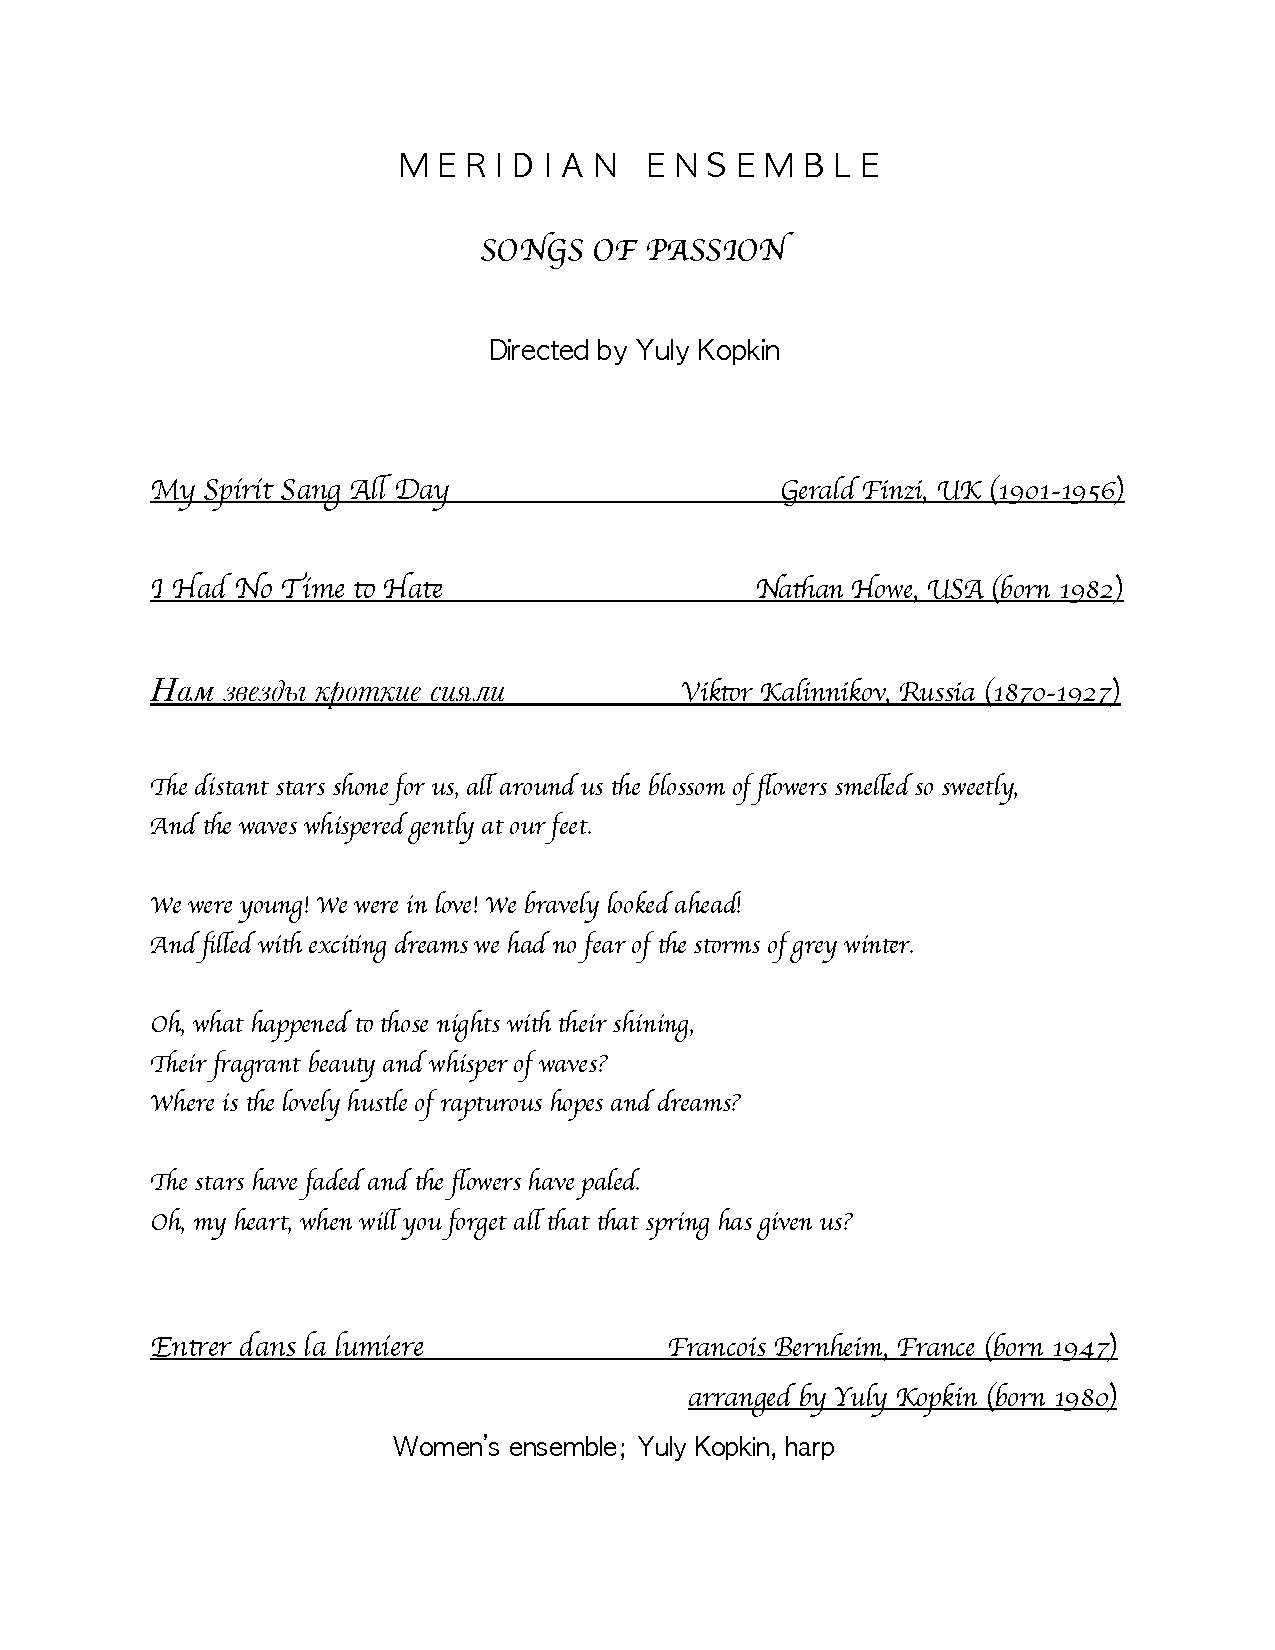
\includegraphics[page=1,natheight=11in,natwidth=8.5in,trim=1in 1in 1in 1in]{ProgramTitles.pdf}%
\hfil%
}%
\vfil
}
\pagebreak
\vbox to \vsize {
\vfil
\hbox to \hsize{
\hfil%
\includegraphics[page=2,natheight=11in,natwidth=8.5in,trim=1in 1in 1in 1in]{ProgramTitles.pdf}%
\hfil%
}%
\vfil
}
\pagebreak
\vbox to \vsize {
\vfil
\hbox to \hsize{
\hfil%
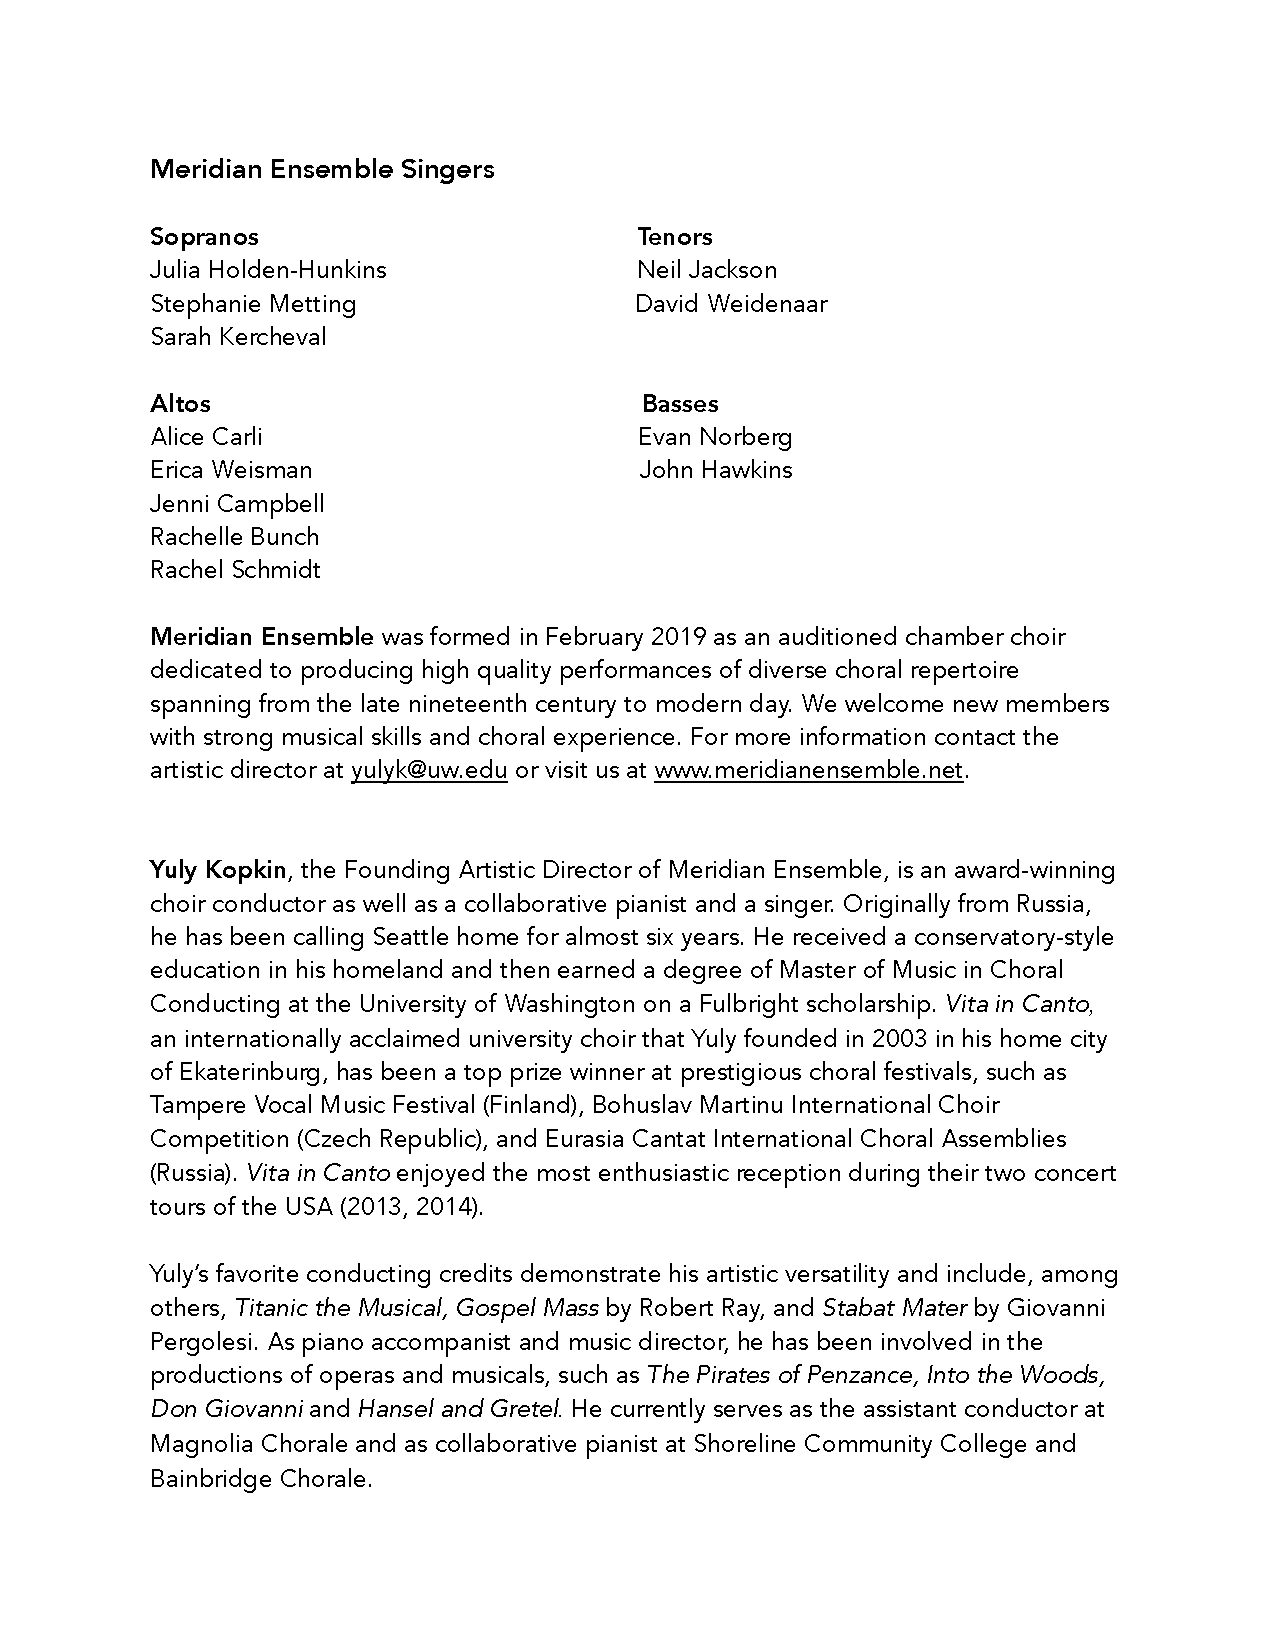
\includegraphics[page=1,natheight=11in,natwidth=8.5in,trim=1in 1in 1in 1in]{About-ensemble-and-director.pdf}%
\hfil%
}%
\vfil
}

% {\centering
    % \fontB{}MERIDIAN ENSEMBLE
    % \vskip 0.2in
    % % \rput[r](-3pt,3pt){\pgfornament[scale=.45]{72}}
    % \fontB{}Songs of Passion%
    % % \rput[l](3pt,3pt){\pgfornament[scale=.45]{73}}\\
    % \vskip 0.4in
    % \fontB{}Directed by Yuly Kopkin%
    % \vskip 0.4in
% }%

% My Spirit Sang All Day\dotfill{}Gerald Finzi, UK (1901\textendash1956)\linebreak

% \bigskip

% I Had No Time To Hate\dotfill{}Nathan Howe, USA (1982\textendash\ )\linebreak

% \bigskip

% Нам звезды кроткие сияли\dotfill{}Viktor Kalinnikov, Russia (1870\textendash1927)\linebreak
% (Nam zyvozdy krotkiye siyali)

% \begin{parcolumns}[rulebetween=true]{2}
% \raggedright%
% \colchunk{Nam zvyozdy krotkiye siyali, chut’ veyal tikhiy veterok.  Krugom tzvety blagauhali, i volny laskovo sheptali u nashikh nok.\vskip\parskip}
% \colchunk{The distant stars shone for us, all around us the blossom of flowers smelled so sweetly,\linebreak{}And the waves whispered gently at our feet.\vskip\parskip}
% \colplacechunks
% \colchunk{this is chunk 2 in column 1}
% \colchunk{this is chunk 2 in column 2}
% \colplacechunks


% \end{parcolumns}



\end{document}